\documentclass[fisica]{fcfmtesis}
%%% opciones: fisica, fisapl, pfa1, pfa2,
%%%           matematicas, lma, actuaria, mem

\usepackage[T1]{fontenc}
\usepackage[utf8]{inputenc}
\usepackage{amsmath,amsfonts,amssymb,amsthm}

\author{Marco Antonio Esperón Pintos}
\title{Aplicación de un regulador cuadrático lineal como método de control en un robot seguidor de líneas}
\asesor{Dr. Jorge Velázquez Castro}
\presidente{Dra. Beatriz Bonilla Capilla}
\secretario{Dr. Andrés Anzo Hernández}
\vocala{Dr. Carlos Arturo Hernández Gracidas}
%\vocalb{}
\date{Febrero de 2019}
\hombre
%\tesina

%%% EJEMPLO de tesis en un solo archivo

\begin{document}

\frontmatter
  \portada
  \maketitle
  \makeacta
  
  \setcounter{page}{4}
  
  \chapter*{Agradecimientos}
  La culminación de una etapa extraordinaria de mi vida no habría sido posible sin el apoyo incondicional de mi familia, por ello quiero agradecer a mi padre Julio Juárez Romero y a mi madre Ma. Mercedes Xochitemol Hernández por confiar en mí cuando decidí estudiar física y perseguir mis sueños; gracias por tantos años de orientación y lecciones de vida, que no les quepa duda que estaré siempre para ustedes así como ustedes lo han estado para mí. A mis hermanos Mónica y José Ubaldo por su cariño y compañía.\\
  
  A Lety y Andy de quienes sólo he recibido la mejor de las amistades, a Mimi que sin su apoyo y constante motivación estas líneas no existirían. A Rogelio y su amistad incondicional.\\
  
  A Lupita por el tiempo y espacio compartido, a Diana por ser un ejemplo a seguir y a mis grandes amigos Levi, Cynthia, Miguel, Rocío, Víctor, Ricardo, Oswaldo, Raúl y Marco con quienes pasé tiempo interminable de alegría. A todos mis amigos y compañeros que hicieron de la facultad mi segunda casa y a quienes tendré siempre en mi memoria.\\
  
  A mi jurado por su valiosa retroalimentación, Dr. Andrés Anzo,  Dra. Beatriz Bonilla, Dr. Carlos Hernández y  Dr. Fernando Rojas.\\
  
  Finalmente le agradezco al Dr. Jorge Velázquez Castro por su paciencia, apoyo y dirección en el desarrollo de este trabajo y de sus enseñanzas en el aula, sin las cuales no tendría claro cuál es el camino profesional que deseo seguir.\\
  
  A todos ustedes, muchas gracias.
  
  \tableofcontents
  \listoffigures
  \listoftables

\chapter{Resumen}
Actualmente la robótica de competición tanto en nuestro país como en el mundo está dominada
por las categorías de robots seguidores de línea y robots sumo; que como el nombre lo sugiere
la primera se trata justamente de la construcción de un robot capaz de seguir una línea dibujada
en el piso a la velocidad más alta posible, mientras que la segunda división consiste en 
construir un robot capaz de rastrear y empujar a su contrincante fuera de un ring circular. La inmensa mayoría de los constructores de robots seguidores han optado por la utilización de control por retroalimentación lineal, como lo es el control PID, ya sea completo o sus variantes PD y PI; esto a causa de ser un control con bibliotecas muy probadas y fáciles de implementar, sin embargo, en las bibliotecas comunes no se contemplan problemas como el \emph{Windup Integrator} o que el ajuste de los parámetros llega a ser complicado; y a pesar de que existen criterios para ajustar los parámetros de ganancia, el ajuste final es mediante prueba y error. En este trabajo se presenta la implementación de un Regulador Cuadrático Lineal (LQR) como alternativa de control al tradicional PID en un robot seguidor de líneas, con el fin de probar la viabilidad de su aplicación en sistemas de mini robótica de competición.\\

\textbf{Palabras clave:} \textsl{Sistema dinámico, Retroalimentación(feedback), Respuesta escalonada(Step Response), Prealimentación(feedforward), Control.}

\chapter{Introducción}
Lorem ipsum dolor sit amet, consectetur adipiscing elit. Nunc fringilla mollis
faucibus. Nunc eleifend imperdiet lorem, a efficitur risus tempus sit amet. Nunc
dolor mauris, maximus sed nibh ac, aliquam ullamcorper odio. Aenean iaculis
neque eget pharetra ultricies. Fusce turpis erat, molestie at vulputate eu,
pellentesque sed ante. Vestibulum ut cursus leo. Duis hendrerit neque et odio
rhoncus aliquam. Morbi tincidunt nunc in ante faucibus, vel pretium purus
accumsan. Suspendisse non malesuada metus. Ut suscipit auctor auctor. Ut
consequat eleifend orci id posuere. Phasellus semper blandit fermentum. Fusce
rhoncus odio et sapien sagittis, non scelerisque sapien interdum. Etiam non ex
hendrerit, congue nulla et, rutrum mauris. Mauris sollicitudin, quam id maximus
aliquet, neque nulla suscipit est, a condimentum magna eros pretium metus. Ut
tempor metus eget massa rutrum commodo \cite{VEI}.

Sed quis lectus porttitor, imperdiet lacus ut, eleifend ex. Ut massa tortor,
auctor vitae suscipit quis, vestibulum id turpis. Maecenas eget erat nisi. Ut
lobortis elementum justo vitae egestas. Integer posuere nisi id tortor commodo
pharetra. Nullam sit amet quam erat. Ut eu ultrices est. Duis facilisis nisl non
metus sagittis vestibulum. Aenean vestibulum nulla condimentum velit interdum,
et congue urna mollis. In consectetur consectetur pellentesque. Vestibulum non
ipsum congue, aliquet lorem vel, viverra augue. Sed blandit ac urna in vehicula.
Ut commodo vehicula tellus sit amet porta.

Esto es una prueba H$_2$. Ésto es otra prueba:
$\mathrm{H}_{\mbox{\scriptsize cualquier cosa}}\mathrm{O}$

\mainmatter
\chapter{Antecedentes}
\section{Anatomía}
Pellentesque habitant morbi tristique senectus et netus et malesuada fames ac
turpis egestas. Morbi eget justo enim. Duis faucibus erat non pellentesque
efficitur. Morbi pretium magna nisl, at porta ligula tristique facilisis. Duis
bibendum risus non vehicula malesuada. Morbi a lacus ex. Nam vulputate porttitor
nulla, eu pretium justo pellentesque nec. In tempus nunc massa, feugiat rhoncus
massa consequat mollis. Fusce id lacus eu nunc bibendum pellentesque \cite{E-Marieb}.

\begin{figure}[!ht]
	\begin{center}
	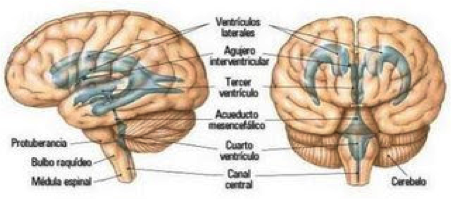
\includegraphics[width=0.6\textwidth]{ventri.png}
	\caption[Ventrículos y ubicación del fluido cerebro espinal]%
	{Ventrículos y ubicación del fluido cerebro espinal \cite{H}}
	\end{center}
\end{figure}

\section{Bla}
In hac habitasse platea dictumst. Mauris non sagittis erat. Nullam ullamcorper
erat metus, ut bibendum lorem egestas id. Nunc accumsan arcu pretium ante
vestibulum, aliquam auctor turpis tristique. Vivamus neque lorem, auctor non
imperdiet at, venenatis sit amet arcu. Mauris sed ante lacus. Etiam sit amet
ipsum ut enim tincidunt lobortis.

\subsection{bla}
Fusce dapibus, eros sed blandit lacinia, quam
mi faucibus dui, a facilisis libero metus sit amet felis. Vestibulum bibendum
nec sem sagittis rutrum. Vivamus porta, odio at dignissim posuere, risus justo
eleifend turpis, sed rutrum ante ipsum sed libero. Phasellus vel tortor faucibus,
sodales lacus eu, euismod enim. Morbi dignissim justo mauris, et tempor neque
suscipit non. Praesent tempor nulla ac dolor venenatis interdum \cite{A}.

\begin{equation}
 IMC=\frac{peso (kg)}{(estatura{}^2 (m) )}
\end{equation}

\chapter{Resultados}
Los resultados del estudio de activaciones BOLD se muestran en la tabla \ref{tab:prueba}.

\begin{table}[h]
	\centering
	\caption{A}
	\label{tab:prueba}
	\begin{tabular}{ccc}
	  a11 & a12 & a13 \\
	  a21 & a22 & a23 \\
	  a31 & a32 & a33
	\end{tabular}
\end{table}

 bla bl bla bla bla bla bla bla bl bla bla bla bla bla bla bla bla bla
 bla bla bla bla bl bla bla bla bla bla bla bl bla bla bla bla bla bla
 bla bla bla bla bla bla bla bl bla bla bla bla bla bla bl bla bla bla
 bla bla bla bl bla bla bla bla bla bla bl bla bla bla bla bla bla bla
 bla bla bla bla

\begin{figure}[h]
	\begin{center}
	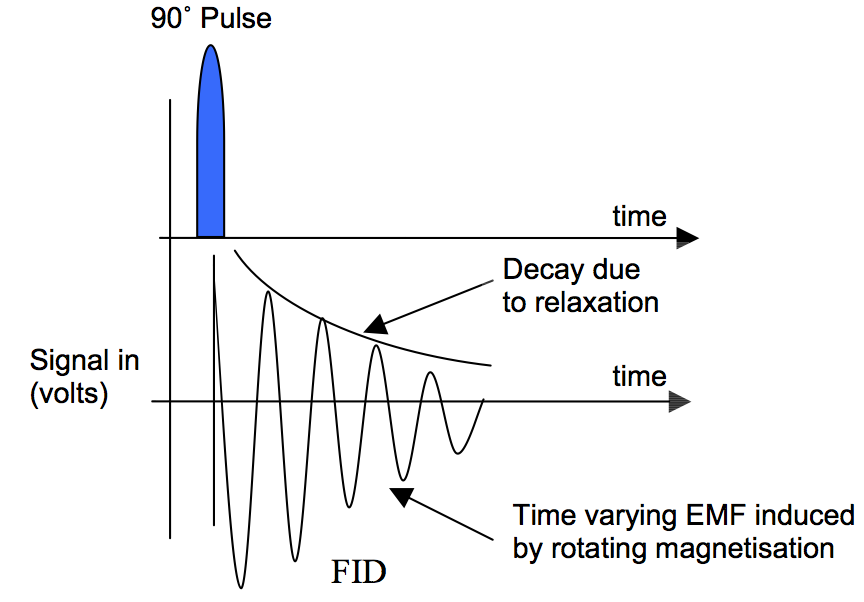
\includegraphics[width=0.8\textwidth]{radiofrec.png}
	\caption{Conexiones}
	\end{center}
\end{figure}

\newpage
\addcontentsline{toc}{chapter}{Conclusión}
\chapter*{Conclusión}

 bla bl bla bla bla bla bla bla bl bla bla bla bla bla bla bla bla bla
 bla bla bla bla bl bla bla bla bla bla bla bl bla bla bla bla bla bla
 bla bla bla bla bla bla bla bl bla bla bla bla bla bla bl bla bla bla
 bla bla bla bl bla bla bla bla bla bla bl bla bla bla bla bla bla bla
 bla bla bla bla

\appendix
\chapter{Bla}

  bla bla bla bla bla bla bla bla bla bla bla bla bla bla bla bla bla bla
  bla bla bla bla bla bla bla bla bla bla bla bla bla bla bla bla bla bla
  bla bla bla bla bla bla bla bla bla bla bla bla bla bla bla bla bla bla
  bla bla bla bla bla bla bla bla bla bla bla bla bla bla bla bla bla bla
  bla bla bla bla bla bla bla bla bla bla bla bla bla bla bla bla bla bla
  bla bla bla bla bla bla bla bla bla bla bla bla bla bla bla bla bla bla
  bla bla bla bla bla bla bla bla bla bla bla bla bla bla bla bla bla bla
  bla bla bla bla bla bla bla bla bla bla bal bla bla bla bla bla bla bla
  bla bla bla bla bla bla bla bla bla bla bla bla bla bla bla bla bla bla
  bla bla bla bla bla bla bla bla bla bla bla bla bla bla bla bla bla bla
  bla bla bla bla bla bla bla bla bla bla bla bla bla bla bla bla bla bla
  bla bla bla bla bla bla bla bla bla bla bla bla bla bla bla bla bla bla
  bla bla bla bla bla bla bla bla bla bla bla bal bla bla bla bla bla bla
  bla bla bla bla bla bla bla bla bla bla bla bla bla bla bla bla bla bla
  bla bla bla bla bla bla bla bla bla bla bla bla bla bla bla bla bla bla
  bla bla bla bla bla bla bla bla bla bla bla bla bla bla bla bla bla bla
  bla bla bla bla bla bla bla bla bla bla bla bla bla bla bla bla bla bla
  bla bla bla bla bla bla bla bla bla bla bla bla bla bla bla bla bla bla
  bla bal bla bla bla bla bla bla bla bla bla bla bla bla bla bla bla bla
  bla bla bla bla bla bla bla bla bla bla bla bla bla bla bla bla bla bla
  bla bla bla bla bla bla bla bla bla bla bla bla bla bla bla bla bla bla
  bla bla bla bla

\backmatter
\addcontentsline{toc}{chapter}{Bibliografía}
\bibliographystyle{plain}
\begin{thebibliography}{99}
	\bibitem{E-Marieb} \textsc{Elaine N. Marieb}, \textit{Essentials of human anatomy and physiology},  novena edición, Pearson, San Franciso, 2009.
	
	\bibitem{H} \textsc{H. Valdivia}, \texttt{www.neurohvp.blogspot.mx}, 14 de Noviembre de 2010.
		
	\bibitem{red} \textsc{REDUCA}, \texttt{www.reeduca.com/neuropsicologia-adul-ninos.aspx}, 22 de Junio de 2009.
	
	\bibitem{John} \textsc{John Oates} y \textsc{Mark Johnson}, \textit{El cerebro en desarrollo},  Child and youth studies group, Reino Unido, 2012.
	
	\bibitem{A} \textsc{A. Gonzalez-Voyer}, \textit{National Library of medicine}, \texttt{www.ncbi.nlm.nih.gov/pmc/?term= brain+structure}, 17 de Diciembre de 2010.
	
	\bibitem{R} \textsc{R. Drake, W. Vogl} y \textsc{A. Michel}, \textit{Gray Anatomía para estudiantes},  novena edición, Elsevier, España, 2007.
	
	\bibitem{Moore} \textsc{Moore Keith, Arthur Dallay} y \textsc{Anne Agur},  \textit{Anatomía con orientación clínica}, sexta edición, Lippincott Williams and Wilkins, Baltimor, USA, 2010.
	
	\bibitem{Nav} \textsc{Ana Navarro},  \textit{Funcionamiento cerebral}, Monografías Neurosicoeducación, 2012.
	
	\bibitem{VEI} \textsc{Veimon} , \textit{Salud siglo XXI}, \texttt{www.elmercaderdelasalud.blogspot.mx/2012/03/trastorno- bipolar-ii.html}, 18 de Marzo de 2012.
\end{thebibliography}

\end{document}
